\section{Superfluidity in liquid helium}
Liquid helium has been found to be an useful liquid to study macroscopic quantum phenomena. This is because helium has a remarkable property of exhibiting superfluidity below $2.17$ K at a pressure of $1$ atm. The temperature of $2.17$ K is commonly known as the Lambda point. Below the Lambda point the behavior of liquid helium is explained by the two-fluid model. According to this model liquid helium has two components, normal fluid component with density $\rho_n$ and superfluid component with density $\rho_s$. 

The phase diagram for helium is shown in Fig. \ref{phaseDiaHe}. The diagram shows that helium is liquid under a broad range of pressure at $0$ K. This fact does not violate the Third law of Thermodynamics since all atoms are in the same quantum state and thus identical. This will make the entropy zero. At $0$ K the entire liquid is superfluid. 
\begin{figure}[H]
\centering 
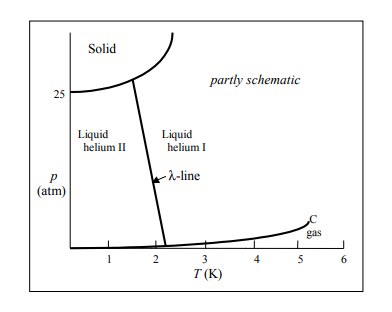
\includegraphics[width=90mm, height=70mm]{Nucleation_Experiment/He_phaseDiagram.png}
\caption{Phase Diagram for $^4He$. \cite{Vinen:808382}}
\label{phaseDiaHe}
\end{figure}

Elementary excitations in liquid helium below the lambda point are in the form of phonons and rotons. These excitations can be explained by studying the plot of energy vs momentum of $^4He$ as shown in Fig. \ref{elementaryExcitation}. This relation is linear at first. Excitations in this region are called phonons and these are high frequency sound waves. The plot has a minimum in energy. The excitations in this region are called rotons and these are excitations with very short wavelengths. Rotons are the ones that make bigger contribution to the specific heat and the thermal energy of Helium at $1$ K and above.
\begin{figure}[H]
\centering 
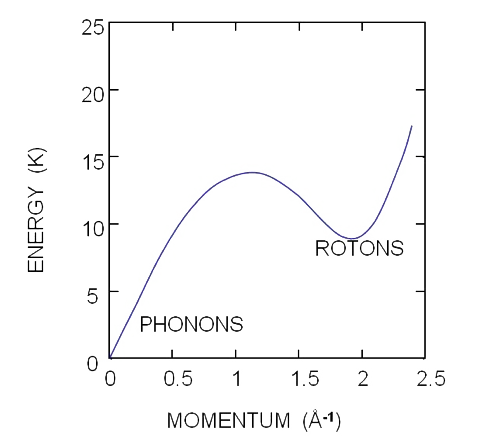
\includegraphics[width=100mm, height=80mm]{Nucleation_Experiment/elementaryexcitations.png}
\caption{Energy versus Momentum for $^4He$. \cite{rotonFig}}
\label{elementaryExcitation}
\end{figure}

Thus helium has a very well studied excitation structure. This fact makes it an ideal liquid to experiment with electron bubbles and study exotic ions. Below the liquid-gas co-existence line, a given state- solid or liquid- can be kept as a metastable state and a phase transition can be introduced only when an energy barrier is overcome. A large nucleus is formed and such a formation is termed homogeneous nucleation. A similar nucleation can be formed at an interface of the helium and impurities, called heterogeneous nucleation.

\section{Nucleation theory}
Nucleation is a general concept that means formation of phase or structure in a homogeneous medium. Cavitation means the nucleation of vapor bubbles in a liquid. To understand cavitation, consider a free vapor bubble in a bulk liquid. The energy required to create such a bubble can be written as the sum of the surface energy of the bubble and the volume energy of the bubble as shown in Eq.\ref{homoBubbleenergyEq}.
\begin{equation}\label{homoBubbleenergyEq}
\Delta E = 4\pi R^2\alpha + \frac{4}{3}\pi R^3\Delta P
\end{equation}
$\alpha$ is the surface tension and $\Delta P = P_{svp} - P_x$ where $P_{svp}$ is the saturated vapor pressure and $P_x$ is the new pressure. A plot of this energy versus radius is shown in Fig. \ref{energyBarrier}.
\begin{figure}[H]
\centering 
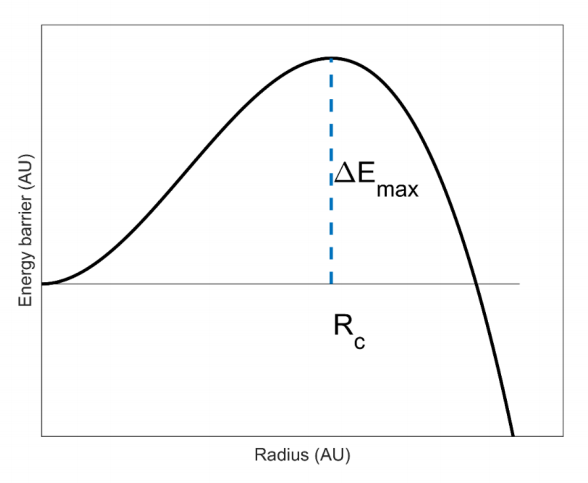
\includegraphics[width=100mm, height=80mm]{Nucleation_Experiment/energyBarrier.png}
\caption{Energy versus Pressure for a gas bubble. \cite{Yang2018thesis}}
\label{energyBarrier}
\end{figure}

Classically, one can obtain the critical radius by differentiating $\Delta E$ with respect to $R$ and setting that to zero. It turns out that
\begin{equation}\label{critRadius}
R_c = \frac{2\alpha}{|\Delta P|}
\end{equation}
Incorporating Eq. \ref{critRadius} into Eq. \ref{homoBubbleenergyEq} we get the energy barrier $\Delta E_{max}$
\begin{equation}\label{energyBarriereq}
\Delta E_{max} = \frac{16\pi \alpha^3}{3|\Delta P|^2}
\end{equation}
Thus a bubble with a radius greater than $R_c$ would grow to a macroscopic size since that is energy favorable. A bubble can be made to reach this critical radius by applying negative pressure by the means of sound waves.

The same calculation can be applied to electron bubbles where the energy is given as:
\begin{equation}\label{energyEq}
E=\frac{h^2}{8mR^2}+4\pi R^2\alpha + \frac{4}{3}\pi R^3 (P-P_{svp})
\end{equation}
The energy versus radius is plotted in Fig. \ref{bubble_energyBarrier} for different values of $\Delta P$.
\begin{figure}[H]
\centering 
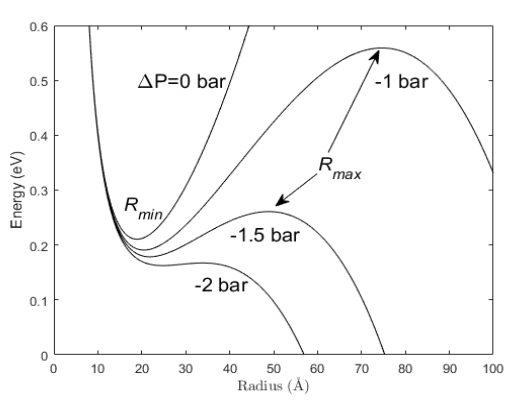
\includegraphics[width=100mm, height=80mm]{Nucleation_Experiment/bubble_energyBarrier.png}
\caption{Energy versus Pressure for an electron bubble. \cite{Yang2018thesis}}
\label{bubble_energyBarrier}
\end{figure}
It is evident that an energy barrier does exist, but only for negative values of $\Delta P$. Otherwise, the electron bubble is stable. Therefore a negative $\Delta P$ is needed in order to nucleate an electron bubble.
Setting $\left.\frac{dE}{dR}\right|_{R_c} = 0$ and $\left.\frac{d^2E}{dR^2}\right|_{R_c} = 0$ we get
\begin{equation}\label{critPresseq}
P_c=-\frac{16}{5}\left(\frac{2\pi m}{5h^2}\right)^{1/4}\alpha^{5/4}
\end{equation}
and
\begin{equation}\label{critRadeq}
R_c = \left(\frac{5h^2}{32\pi m\alpha}\right)^{1/4}
\end{equation}
The experiment is used to verify that the critical pressure agrees with the theoretical formula given by Eq. \ref{critPresseq}. Then the same experiment can be performed to find the critical radius and critical pressure for exotic ions where there is no theoretical prediction.

\section{Heterogeneous nucleation}
There are at least three types of heterogeneous nucleation. The first type being from normal electron bubbles produced by introducing a radioactive beta source. The electrons from the source can also excite helium atoms and cause the second kind of heterogeneous nucleation. In this process, the excited helium atoms get ionized and the resultant electron is called a secondary electron. This electron would be quickly pulled backed to the positive ion due to electrostatic force; however, before recombination the electron can form a bubble and be cavitated. The third one is due to a process called Penning ionization. After the recombination, a helium atom is in an excited state and will combine with another helium atom in the ground state to form a dimer.
$$He^*+He\rightarrow He^*_2$$
Then by Penning ionization process, two dimers can be annihilated.
\begin{equation}\label{HeliumEq1}
He^*_2+He^*_2 \rightarrow 3He +He^+ + e^-
\end{equation}
or
\begin{equation}\label{HeliumEq2}
He^*_2+He^*_2 \rightarrow 2He + He^+_2 + e^-
\end{equation}
Thus in principle, there should be two different thresholds for cavitation by electrons. The first one due to electrons coming from the beta source. The second one is due to secondary electrons and electrons due to the Penning ionization process. Classen et al \cite{Classen} reported two different thresholds for cavitation by electrons when they conducted experiments with a thallium source. They reported two different critical pressures at which the nucleations were observed. The first one $|P_{rare}|$ was due to electrons from the source and the second was due to the secondary electrons $|P_{secondary}|$. There was a third new critical pressure between these pressures. The events due to this were termed rare events since the probability of them was very low. Our experiments suggest that $|P_{secondary}| = |P_{dimers}|$.
\section{Experimental setup}
The cryostat structure is shown in Fig. \ref{cryostatfig}. The bubbles are nucleated in a piezoelectric transducer located inside the cell. There are several baths to cool the cryostat. Liquid nitrogen baths are located towards the outside and have their own pumping lines. The helium baths are on the top and are filled with liquid helium. In order to have extreme purity inside the cell, ultra pure helium gas is liquidized using the helium baths. This cooling power comes from the evaporation of liquid in the helium baths. Then the top of each helium bath is pumped. The evaporating helium from the baths will absorb heat from the pumping lines that contain the ultra pure gas. Ultimately, this gas would liquidify and fill the cell. 

While using $^4He$, temperatures as low as $1$ K can be reached by using this process. The second pot is used to provide thermal anchoring for the main pot. There was a radioactive $\beta$ source on top of the transducer that introduced electrons to the cell. In order to study homogeneous nucleation, a potential is applied between the transducer and the source. If $\Delta$V is negative, the electrons would not arrive at the transducer and the nucleation would then be because of secondary electrons and as a result of the Penning ionization process.
\begin{figure}[H]
\centering 
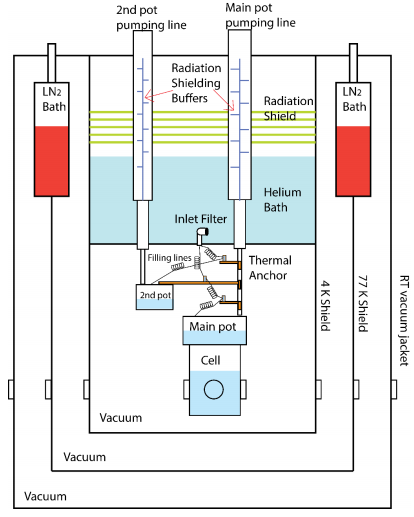
\includegraphics[width=90mm, height=120mm]{Nucleation_Experiment/cryostat.png}
\caption{Design of the cryostat. \cite{Yang2018thesis}}
\label{cryostatfig}
\end{figure}
The transducer had an outer diameter of $2.54$ cm and a thickness of $0.49$ cm. It had two resonance frequencies at $115$ kHz and $471$ kHz. When the transducer is operated at $115$ kHz, it is said to be operated on a flexural mode, and when it is operated at $471$ kHz, it is said to be operated on a thickness mode. The names come from the fact that the transducer vibrates with different mechanisms at each of the two frequencies. 

The sound waves produced by the transducer would collect at the focus and that is where the nucleation is observed. The focus is targeted by a laser beam of wavelength $532$ nm and a power of about $30$ mW. A lens is used to converge the laser at the focus. 

If an electron bubble were present at the focus, the laser would be scattered by it. This scattered light is then converged onto a PMT detector using another lens. During the experiment, $300$ pulses are sent to the transducer and the number of pulses detected by the PMT are recorded. This will give the probability of nucleation at a given temperature.
\begin{figure}[H]
\centering 
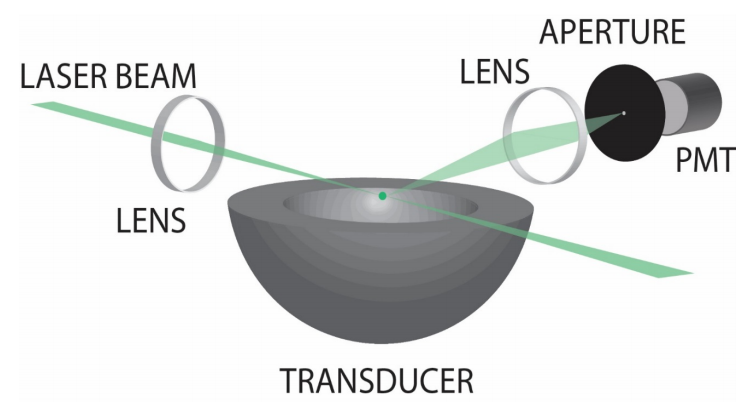
\includegraphics[width=100mm, height=50mm]{Nucleation_Experiment/experimental_setup.png}
\caption{A schematic showing working of the laser to detect nucleation. \cite{Yang2018}}
\label{laserSetup}
\end{figure}
\section{Results}
Figure \ref{probVoltage} shows the probability versus the voltage on the transducer. The two different thresholds are evident. Switching the voltage meant that the electrons from the radioactive source no longer reached the transducer. We know the nucleation events with the smaller threshold are from secondary electrons and the Penning ionization process. A low probability tail is observed in the curve. These events, with low threshold and low probability, are not explained by theory and are called very rare events.
\begin{figure}[H]
\centering 
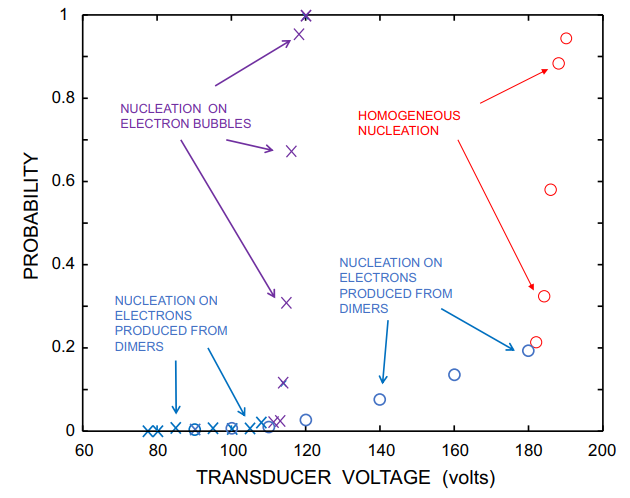
\includegraphics[width=100mm, height=80mm]{Nucleation_Experiment/probVsVoltage.png}
\caption{Probability of nucleation versus the voltage on transducer at $2.5$ K temperature and $0.42$ bar static pressure. The crosses represent data taken with $-200$ V on the source and the circles represent data with $+200V$ on the source. \cite{Yang2018}}
\label{probVoltage}
\end{figure}

It is possible that the rare events and very rare events are a result of nucleation of dust in the cell. Yang et all \cite{Yang2018thesis} conducted a separate experiment with a tip that was coated with carbon nanotubes as an electron source and produced the same results. Thus the rare events and very rare events are indeed related to electrons.

In order to study the rare events more carefully, we conducted experiments with a Thallium source. This is done because the number density of electrons is smaller for a Thallium source. Therefore the probability increases gradually with transducer voltage and we can study the rare events and very rare events carefully. Figure \ref{probVoltageThallium} shows the results with the Thallium source. It is clear that rare events are different than very rare events.
\begin{figure}[H]
\centering 
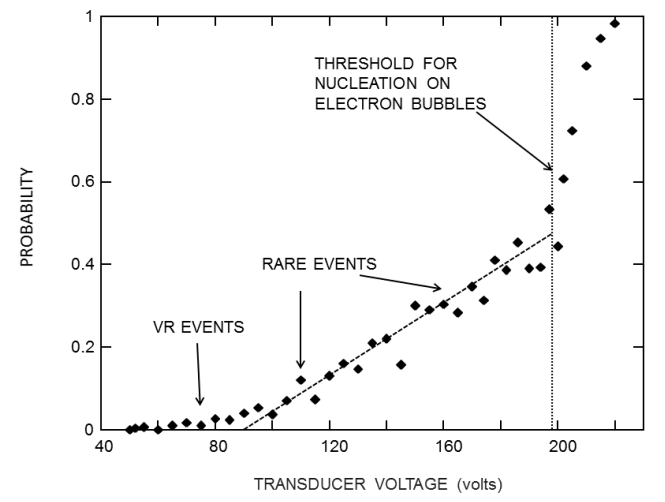
\includegraphics[width=100mm, height=80mm]{Nucleation_Experiment/thalliumSource.png}
\caption{Results using Thallium source \cite{Yang2018thesis}. The dashed line shows the threshold for caviation of electron the source. The data was taken at $3.00$ K temperature and $0.34$ bar static pressure.}
\label{probVoltageThallium}
\end{figure}
Below a certain voltage, the electrons from the source will not cavitate and the rare events will manifest in the probability voltage plot. The secondary electrons and penning ionization provide an explanation for rare events; however, not much is known about the very rare events.
\section{Deviation from prediction}
It was investigated how the threshold voltage discussed in the previous section varies with different temperatures and static pressures. The transducer was in thickness mode. As seen in Fig. \ref{non_linear1}, the variation against static pressure at a constant temperature is linear.
\begin{figure}[H]
\centering 
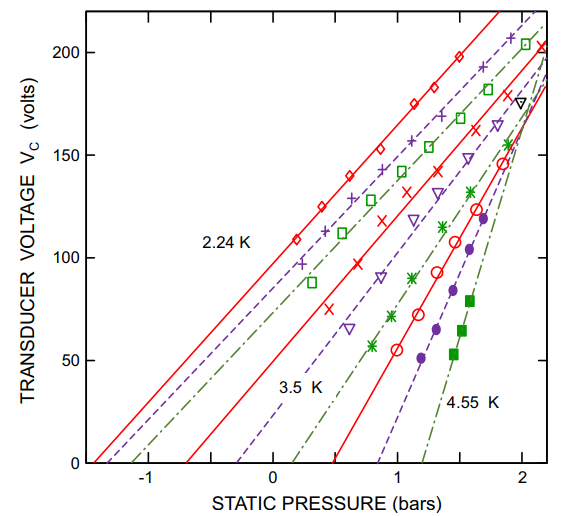
\includegraphics[width=100mm, height=80mm]{Nucleation_Experiment/non_linear1.PNG}
\caption{Threshold voltages for electron bubbles against static pressure for different temperatures. \cite{Yang2018thesis}}
\label{non_linear1}
\end{figure}

Thus the threshold voltage, $V_c$ can be written as
\begin{equation}\label{threshVoltageEq}
V_c=aP_{stat}+b
\end{equation}
Setting $V_c=0$, we can find the critical pressure $P_{el}$. This pressure is the static pressure which alone can produce cavitation in electron bubbles without the transducer. By linear fitting the data, we found the $P_{el}$ for different temperatures. The result is shown in Fig. \ref{non_linear2}. For comparison, we have also shown the data taken by Classen et al. \cite{Classen}
\begin{figure}[H]
\centering 
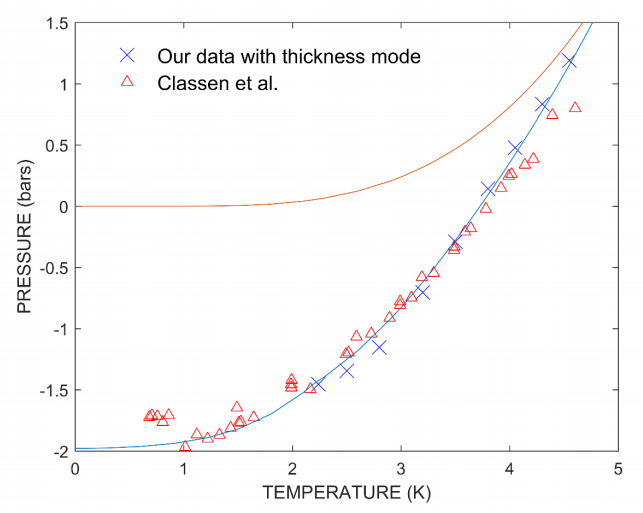
\includegraphics[width=100mm, height=80mm]{Nucleation_Experiment/non_linear2.png}
\caption{Critical pressure for nucleation versus temperature. The blue curve is the theoretical prediction by Eq. \ref{critPresseq}. The triangle points are from Classen et al. \cite{Classen} The yellow solid curve shows the saturated vapor pressure. \cite{Classen} \cite{Yang2018thesis}}
\label{non_linear2}
\end{figure}

Experimental data seems to agree quite well with that taken by Classen et al \cite{Classen} and the theoretical prediction for temperatures greater than $1$ K. Below $1$ K, they seem to be diverging from the expected value. Classen et al \cite{Classen} did not observe this since they did not collect data around $1$ K. It was also noted that the critical pressures measured with the flexural mode was always less negative than one with the thickness mode. One possible explanation is the sound waves in liquid helium have a nonlinear propagation. The sound might be getting distorted as it propagates due to nonlinearities in Helium. This would mean that the pressure at the focus might not be the same as the pressure at which we drive the transducer. This would especially be more prominent as the amplitude increases. We explore this possibility using simulations in the next chapter.